%%%%%%%%%%%%%%%%%%%%%%%%%%%%%%%%%%%%%%%%%
% University/School Laboratory Report
% LaTeX Template
% Version 3.1 (25/3/14)
%
% This template has been downloaded from:
% http://www.LaTeXTemplates.com
%
% Original author:
% Linux and Unix Users Group at Virginia Tech Wiki 
% (https://vtluug.org/wiki/Example_LaTeX_chem_lab_report)
%
% License:
% CC BY-NC-SA 3.0 (http://creativecommons.org/licenses/by-nc-sa/3.0/)
%
%%%%%%%%%%%%%%%%%%%%%%%%%%%%%%%%%%%%%%%%%

%----------------------------------------------------------------------------------------
%	PACKAGES AND DOCUMENT CONFIGURATIONS
%----------------------------------------------------------------------------------------

\documentclass{article}

\usepackage[version=3]{mhchem} % Package for chemical equation typesetting
%\usepackage{siunitx} % Provides the \SI{}{} and \si{} command for typesetting SI units
\usepackage{graphicx} % Required for the inclusion of images
\usepackage{natbib} % Required to change bibliography style to APA
\usepackage{amsmath} % Required for some math elements 
\usepackage{hyperref}
 \usepackage{pdflscape}
\usepackage[a4paper,margin=0.5in]{geometry}
\setlength\parindent{0pt} % Removes all indentation from paragraphs

\renewcommand{\labelenumi}{\alph{enumi}.} % Make numbering in the enumerate environment by letter rather than number (e.g. section 6)

%\usepackage{times} % Uncomment to use the Times New Roman font

%----------------------------------------------------------------------------------------
%	DOCUMENT INFORMATION
%----------------------------------------------------------------------------------------

\title{Gate Detection} % Title

\author{Philipp \textsc{Duernay}} % Author name

\date{\today} % Date for the report

\begin{document}
\maketitle
% If you wish to include an abstract, uncomment the lines below
% \begin{abstract}
% Abstract text
% \end{abstract}

%----------------------------------------------------------------------------------------
%	SECTION 1
%----------------------------------------------------------------------------------------

\section{Recap}
In the last meeting from 25.07.2018 several next steps were defined:
\begin{itemize}
	\item Write it all down.
	\item Add prediction layers at multiple scales
	\item Investigate performance in terms of occlusion/angle
	\item Remove/Reduce occlusions from the dataset and repeat experiments. We could use the drone model we created for testing the filters to simulate the flight of a real drone and record the images.
	
\end{itemize}

\section{Prediction Layers at multiple scales}

Last experiments showed how having predicting layers at multiple scales at the end of the network improved the predictions for larger objects. So I did some experiments alternating the amount of prediction layers and their scales \autoref{fig:scales}.

\begin{figure}[htbp]
	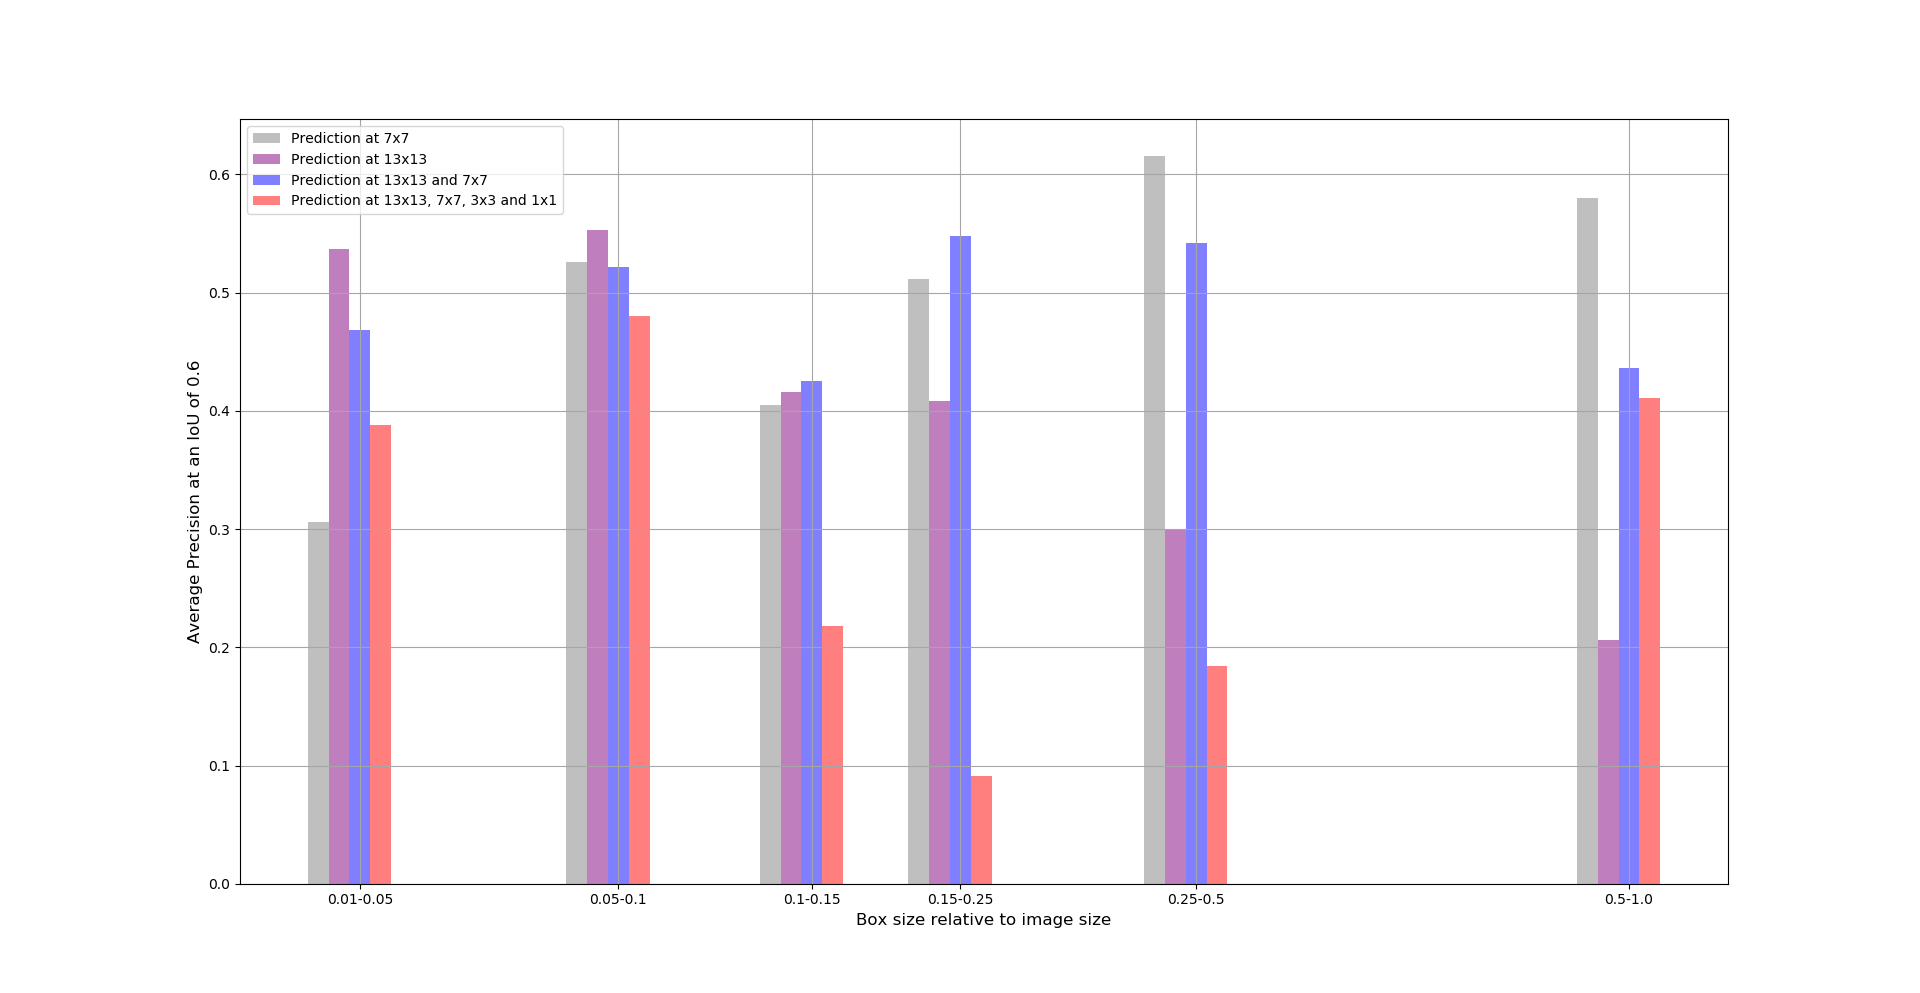
\includegraphics[width=\linewidth]{area}
	\caption{Average Precision for different box sizes on a test set of 1000 images.}
	\label{fig:scales}
\end{figure}

\section{Dataset Generation}

In the last dataset it looked like a lot of gates were only party visible so I created a new dataset using Shuo's drone model + velocity controller.

\section{Training on new data.}



\section{Next Steps}
\begin{itemize}
	\item Write it all down.
	\item Add prediction layers at multiple scales
	\item Investigate performance in terms of occlusion/angle
	\item Remove/Reduce occlusions from the dataset and repeat experiments. We could use the drone model we created for testing the filters to simulate the flight of a real drone and record the images.

\end{itemize}


\end{document}\grid
